\documentclass[11pt,a4paper]{article}

\usepackage[margin=1in]{geometry}
\usepackage{titlesec}
\usepackage{enumitem}
\usepackage{hyperref}
\usepackage{parskip}
\usepackage{graphicx}
\usepackage{float}
\usepackage{booktabs}
\usepackage{amsmath}

\hypersetup{colorlinks=true, linkcolor=blue, urlcolor=blue}

\titleformat{\section}{\large\bfseries}{\thesection}{0.5em}{}
\titleformat{\subsection}{\normalsize\bfseries}{\thesubsection}{0.5em}{}
\setlist{leftmargin=1.4em, topsep=2pt, itemsep=2pt}

\title{\vspace{-1.5cm}\textbf{PKCERT AI \& Software Development Internship \\ Task 17: Neural Network Fundamentals}}
\author{Abdullah Amir}
\date{AI and Software Development \\ 27 July 2026}

\begin{document}

\maketitle
\vspace{-0.8cm}

This report covers the theory, derivations and results. The full code and outputs live
in the notebook \texttt{neural\_network\_fundamentals.ipynb}. Every core computation --
the perceptron's learning rule, the five activation functions and their derivatives,
and the 2-layer network's forward and backward passes -- is implemented in plain NumPy;
no autograd framework computes a gradient anywhere in this submission. scikit-learn
appears only for the permitted \texttt{MLPClassifier} baseline and for ordinary
preprocessing/evaluation utilities.

% ----------------------------------------------------------------
\section*{Part A: Perceptron Fundamentals}

A single-layer perceptron with a hard step activation, trained with the classic rule
$w \leftarrow w + \eta(y - \hat y)x$, updated one misclassified sample at a time.

\textbf{A linearly separable case.} Setosa vs Versicolor from Iris, using petal length
and width. The perceptron converged in \textbf{2 epochs} (2 errors in epoch 1, 0 in
epoch 2), reaching 100\% training accuracy.

\begin{figure}[H]
    \centering
    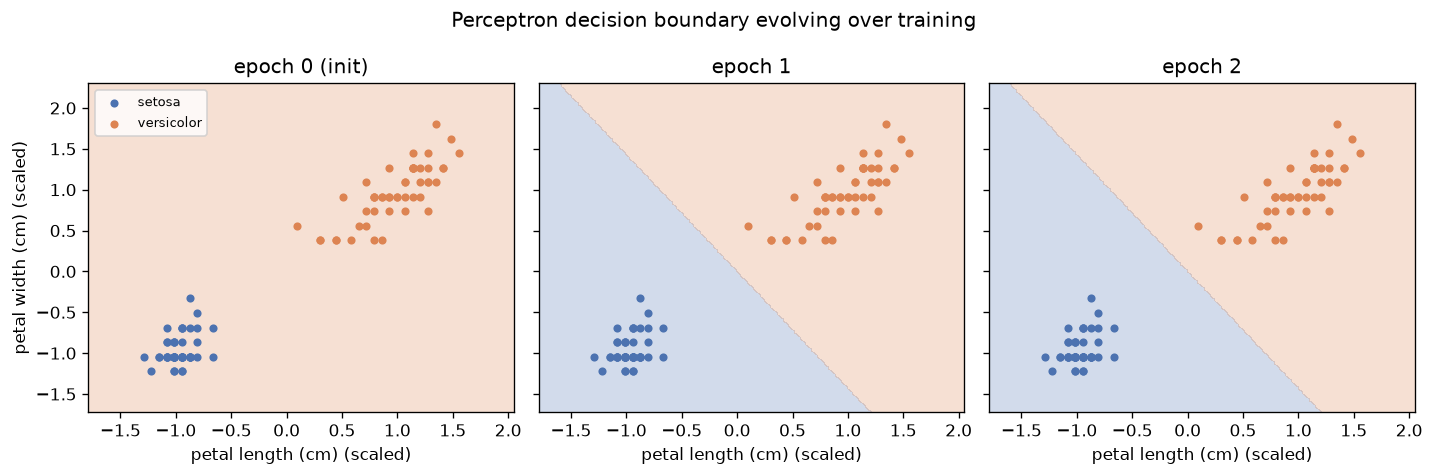
\includegraphics[width=0.95\textwidth]{figures/01_perceptron_boundary_evolution.png}
    \caption{The decision boundary at initialisation, after 1 epoch, and after 2 (converged).}
\end{figure}

\textbf{A non-linearly separable case: XOR.} The identical algorithm, given XOR's 4
points, ran the full 50 epochs without ever reaching zero errors, plateauing at 4/4
misclassifications and 50\% training accuracy -- chance level.

\begin{figure}[H]
    \centering
    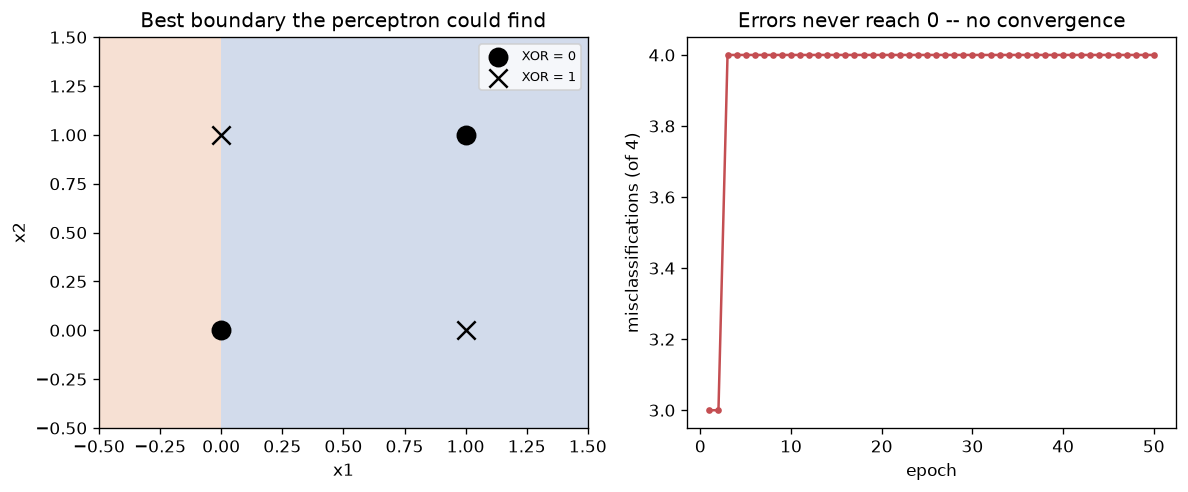
\includegraphics[width=0.85\textwidth]{figures/02_perceptron_xor_failure.png}
    \caption{Left: the best single straight-line boundary the perceptron could find.
    Right: the error count never falls, unlike the Iris case above.}
\end{figure}

\textbf{Why XOR defeats a single perceptron.} A perceptron's decision boundary is one
hyperplane, $w \cdot x + b = 0$. XOR's four points require two separate diagonal
boundaries -- $(0,0)$ and $(1,1)$ on one side, $(0,1)$ and $(1,0)$ on the other -- which
is not a linearly separable arrangement. No choice of $w, b$ places a single straight
line between the two classes, exactly what the flat, non-decreasing error curve shows:
the rule keeps correcting one misclassified point only to break another.

\textbf{Perceptron vs logistic regression.} Both are linear classifiers computing the
identical score $z = w \cdot x + b$ and both learn by adjusting $w, b$ from labelled
examples; they differ in what happens to $z$ and how that drives learning. The
perceptron applies a hard step (predict 1 if $z \ge 0$) and updates weights only on
misclassified points, by an amount proportional to the raw error
$(y-\hat y) \in \{-1,0,1\}$ -- a mistake-driven rule with no smooth loss surface.
Logistic regression applies the smooth sigmoid to $z$ to obtain a probability, defines
cross-entropy loss over it, and updates every point's weights by gradient descent on
that loss, whose gradient takes the strikingly similar form $(y-p)x$ -- except $p$ is a
continuous probability, not a hard vote. As the sigmoid's steepness goes to infinity,
logistic regression's smooth boundary collapses into the perceptron's hard one: the
perceptron is, informally, the hard-threshold, mistake-driven special case of the same
linear model that logistic regression fits with a smooth, probabilistic loss.

% ----------------------------------------------------------------
\section*{Part B: Activation Functions}

Sigmoid, Tanh, ReLU and Leaky ReLU, plotted with their derivatives over $[-10,10]$.

\begin{figure}[H]
    \centering
    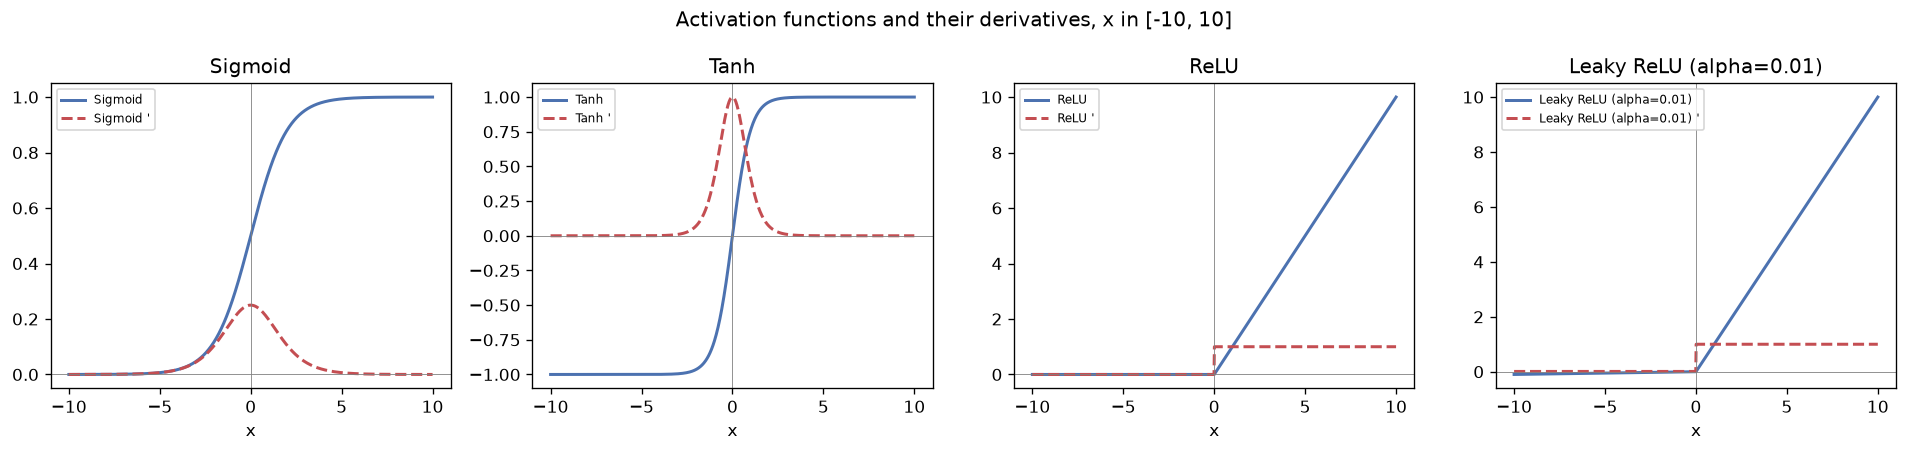
\includegraphics[width=0.95\textwidth]{figures/03_activation_functions.png}
    \caption{Each function (solid) and its derivative (dashed).}
\end{figure}

Softmax is not elementwise -- every output depends on every logit, and its true
derivative is a Jacobian, not a single curve -- so it is shown instead by sweeping one
logit while the other two are held fixed.

\begin{figure}[H]
    \centering
    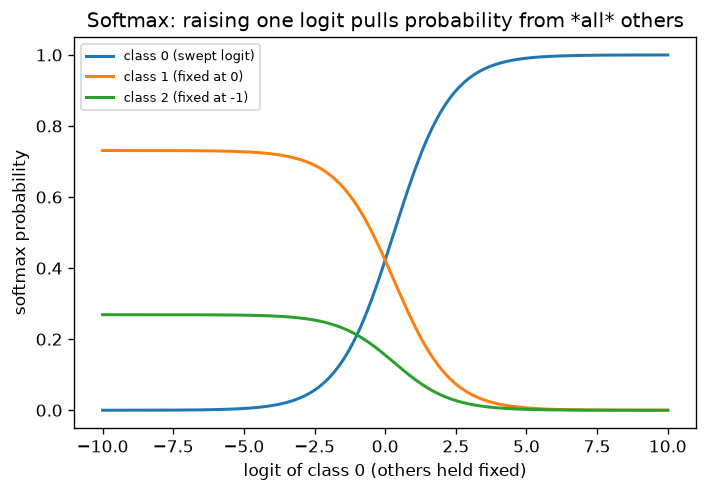
\includegraphics[width=0.68\textwidth]{figures/03b_softmax_behaviour.png}
    \caption{Raising one logit pulls probability mass from \emph{every} other class,
    not just proportionally -- the class fixed at logit 0 (orange) loses more
    probability than the class fixed at $-1$ (green) as class 0's logit rises.}
\end{figure}

\textbf{Vanishing gradient.} Backpropagation multiplies the upstream gradient by each
layer's activation derivative (chain rule), so a deep stack multiplies many such
derivatives together. Sigmoid's derivative peaks at only \textbf{0.25} (at $x=0$) and is
already below 0.01 by $|x| \approx 4.6$; tanh peaks higher, at \textbf{1.0}, but still
decays toward 0 beyond $|x|\approx 3$. Across the full $[-10,10]$ range tested, the
derivative sits below $10^{-3}$ for \textbf{31.0\%} of sigmoid's domain and
\textbf{58.6\%} of tanh's. Stacking several sigmoid or tanh layers multiplies together
numbers mostly well below 1, and the product shrinks toward 0 exponentially with depth
-- the vanishing gradient problem. Sigmoid is the more susceptible of the two, both
because its peak derivative is four times smaller and because its outputs are never
centred on 0. ReLU's derivative is exactly 1 for any $x>0$, passing gradient through
unchanged no matter how deep the stack -- the main reason it replaced sigmoid/tanh as
the default hidden-layer choice in deep networks.

\textbf{Dying ReLU vs Leaky ReLU.} ReLU's derivative is exactly 0 for every $x<0$. If a
neuron's weighted input lands below 0 for every training example, every future gradient
through it is also exactly 0: its weights stop updating and it is permanently dead.
Leaky ReLU fixes this with one change -- scaling negative inputs by a small constant
$\alpha=0.01$ instead of clamping to 0 -- so the derivative on the negative side is
$\alpha$, not 0. A leaky-ReLU neuron that lands in negative territory still receives a
small gradient and can recover; it can never become permanently dead the way a plain
ReLU neuron can.

\textbf{Hidden layer vs output layer, multi-class classification.} ReLU (or Leaky ReLU)
is the standard hidden-layer choice: cheap, no positive-side saturation, avoids the
vanishing-gradient slowdown demonstrated above. Softmax is the right output-layer choice
because it is the only one of the five that guarantees a valid probability
distribution -- every output in $[0,1]$, all summing to exactly 1 -- and it pairs with
cross-entropy loss to give the clean gradient used directly in Part C.

% ----------------------------------------------------------------
\section*{Part C: Forward \& Backpropagation Mini-Project}

\textbf{Dataset.} Palmer Penguins (Gorman, Williams \& Fraser, 2014): 4 numeric
measurements (\texttt{bill\_length\_mm}, \texttt{bill\_depth\_mm},
\texttt{flipper\_length\_mm}, \texttt{body\_mass\_g}), 3 species (Adelie, Chinstrap,
Gentoo), 342 penguins after dropping rows with a missing measurement. Not used in any
earlier task, and a natural fit for the required 2--4 input features / 2--4 output
classes.

\subsection*{Derivation (matrix form)}

Architecture: $X\,(N,d) \to [W_1,b_1] \to Z_1 \to \text{ReLU} \to A_1 \to [W_2,b_2] \to
Z_2 \to \text{softmax} \to A_2$, with $d=4$, $h=8$ hidden units, $c=3$.

\textbf{Forward:}
\[
Z_1 = XW_1 + b_1 \qquad A_1 = \text{ReLU}(Z_1) \qquad Z_2 = A_1 W_2 + b_2 \qquad A_2 = \text{softmax}(Z_2)
\]

\textbf{Loss} (mean categorical cross-entropy, $Y$ one-hot):
\[
L = -\frac{1}{N}\sum_{n=1}^{N}\sum_{k=1}^{c} Y_{nk}\log(A_{2,nk})
\]

\textbf{Backward.} The softmax+cross-entropy pair has a well-known closed-form first
gradient ($\partial L/\partial Z_{2,j} = A_{2,j} - Y_j$ per example); batched and
pre-divided by $N$:
\[
dZ_2 = \frac{A_2 - Y}{N} \qquad dW_2 = A_1^\top dZ_2 \qquad db_2 = \textstyle\sum_n dZ_2
\]
\[
dA_1 = dZ_2 W_2^\top \qquad dZ_1 = dA_1 \odot \text{ReLU}'(Z_1) \qquad dW_1 = X^\top dZ_1 \qquad db_1 = \textstyle\sum_n dZ_1
\]

\textbf{Update:} $W \leftarrow W - \eta\,dW$, $\;b \leftarrow b - \eta\,db$.

\subsection*{Gradient check}

Before trusting anything trained with this derivation, its analytical gradients were
checked against numerical (finite-difference) gradients on six random entries of each
parameter matrix -- the standard, and only truly convincing, way to catch a sign error
or a transposed matrix in a hand-derived backward pass.

\begin{table}[H]
\centering
\begin{tabular}{lr}
\toprule
\textbf{Parameter} & \textbf{Max relative error (analytical vs numerical)} \\
\midrule
$W_1$ & $5.15\times10^{-11}$ \\
$b_1$ & $1.03\times10^{-10}$ \\
$W_2$ & $3.18\times10^{-11}$ \\
$b_2$ & $2.26\times10^{-11}$ \\
\bottomrule
\end{tabular}
\caption{All four pass at $\sim 10^{-10}$--$10^{-11}$, essentially floating-point noise
rather than approximation error (threshold for a pass: $10^{-5}$).}
\end{table}

\subsection*{Training and results}

Trained with mini-batch gradient descent (batch size 16, 300 epochs, learning rate 0.1,
He-initialised weights).

\begin{figure}[H]
    \centering
    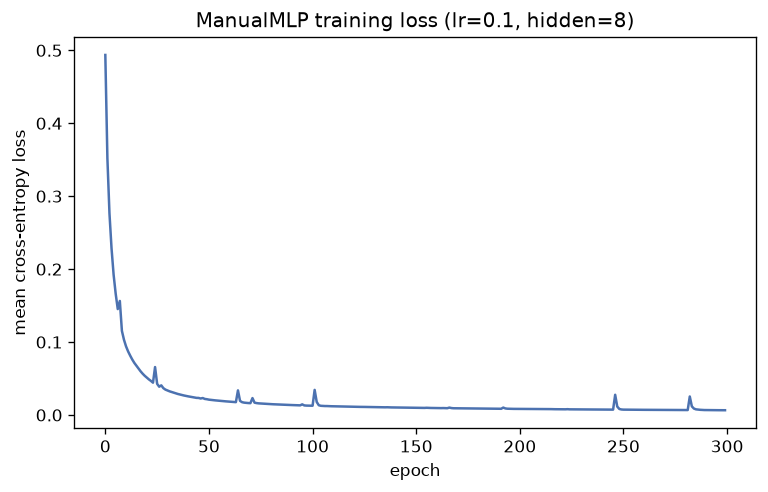
\includegraphics[width=0.62\textwidth]{figures/04_loss_curve.png}
    \caption{Training loss, ManualMLP.}
\end{figure}

\begin{table}[H]
\centering
\begin{tabular}{lrrrr}
\toprule
\textbf{Model} & \textbf{Accuracy} & \textbf{Macro-Precision} & \textbf{Macro-Recall} & \textbf{Macro-F1} \\
\midrule
ManualMLP (from-scratch NumPy) & 0.9855 & 0.9892 & 0.9867 & 0.9877 \\
sklearn MLPClassifier (same architecture) & \textbf{1.0000} & \textbf{1.0000} & \textbf{1.0000} & \textbf{1.0000} \\
\bottomrule
\end{tabular}
\caption{Test set (69 penguins), macro-averaged across 3 classes.}
\end{table}

\begin{figure}[H]
    \centering
    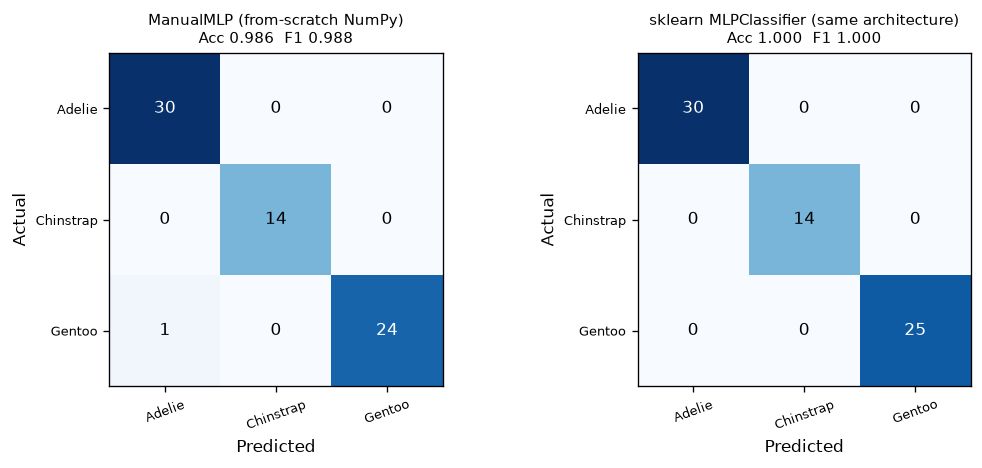
\includegraphics[width=0.95\textwidth]{figures/05_confusion_matrices.png}
    \caption{ManualMLP misclassifies exactly one Gentoo penguin as Adelie;
    sklearn's baseline gets a perfect confusion matrix on this split.}
\end{figure}

\textbf{The from-scratch network is competitive with the framework baseline, not
merely functional.} A 1.45-percentage-point accuracy gap on a 69-row test set is a
single misclassified penguin -- consistent with ordinary training-run variance (different
weight initialisation, SGD's stochastic batch order) rather than any structural
shortcoming in the hand-derived math, which the gradient check above already confirmed
independently.

\begin{figure}[H]
    \centering
    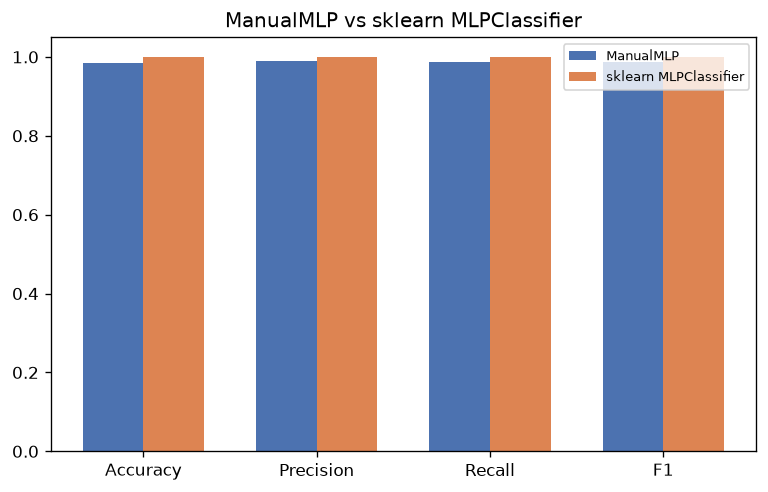
\includegraphics[width=0.62\textwidth]{figures/06_metrics_comparison.png}
    \caption{Every metric tracks the same near-tie shown in the table above.}
\end{figure}

\subsection*{Hyperparameter experiment: learning rate}

\begin{table}[H]
\centering
\begin{tabular}{lrr}
\toprule
\textbf{Learning rate} & \textbf{Final training loss} & \textbf{Test accuracy} \\
\midrule
0.001 & 0.2694 & 0.8841 \\
0.01  & 0.0346 & \textbf{1.0000} \\
0.1   & 0.0065 & 0.9855 \\
1.0   & \textbf{0.0021} & 0.9855 \\
\bottomrule
\end{tabular}
\end{table}

\begin{figure}[H]
    \centering
    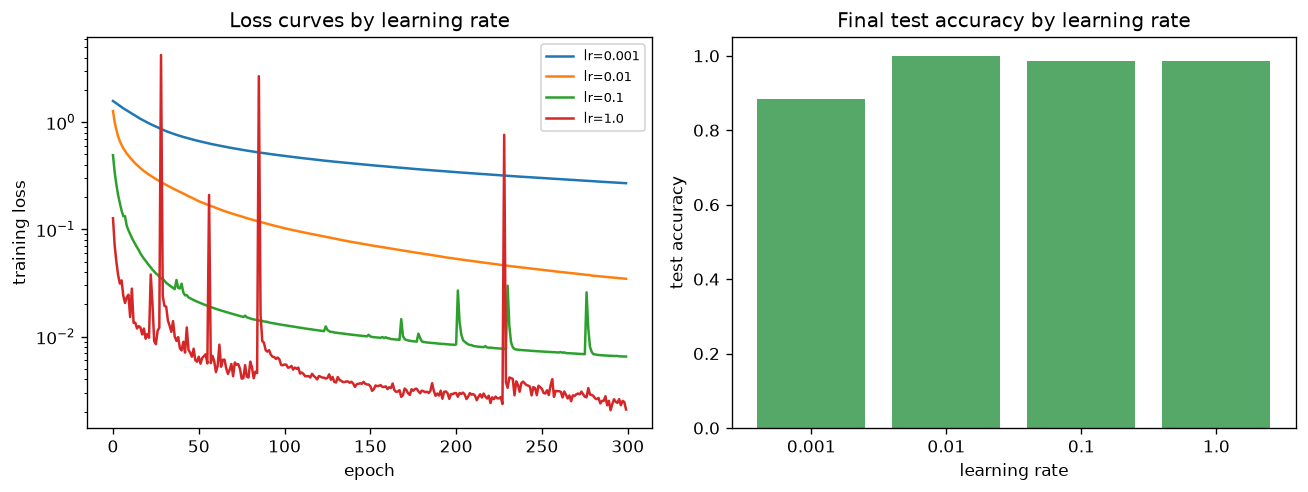
\includegraphics[width=0.95\textwidth]{figures/07_lr_experiment.png}
    \caption{Left: loss curves (log scale) by learning rate. Right: final test accuracy.}
\end{figure}

\textbf{Reading the experiment.} \texttt{lr=0.001} is visibly under-converged after 300
epochs (smooth but still high loss, 88.4\% test accuracy) -- too slow. \texttt{lr=0.01}
converges smoothly to a low loss and reaches \textbf{100\% test accuracy}, the sweet
spot on this problem. \texttt{lr=0.1} and \texttt{lr=1.0} both show sharp periodic
spikes in the loss curve, visible even on a log scale -- the signature of steps large
enough to occasionally overshoot a good minimum before settling back down.
\texttt{lr=1.0} reaches the \emph{lowest} final training loss of all four but does not
translate into the best test accuracy, which is the concrete, checked version of the
general warning against tuning purely on training loss.

% ----------------------------------------------------------------
\section*{Part D: Analysis \& Documentation}

\textbf{Pipeline summary.} A 2-layer MLP, $4 \to 8 \to 3$: 4 standardised numeric
penguin measurements in, one hidden layer of 8 units with \textbf{ReLU} (the
Part-B-justified standard hidden-layer default), an output layer of 3 units with
\textbf{softmax} (the only function studied that yields a valid probability
distribution, and the one whose gradient combines cleanly with cross-entropy). Trained
with mini-batch gradient descent, He-initialised weights, for 300 epochs. The trained
$\{W_1, b_1, W_2, b_2\}$ are saved with \texttt{pickle} to
\texttt{manual\_mlp\_params.pkl}; reloading them was verified to reproduce identical
test-set predictions.

\textbf{Hyperparameter experiment findings.} See above: learning rate shows a clear
too-slow / sweet-spot / too-noisy progression, and the lowest training loss
(\texttt{lr=1.0}) was not the best-generalising choice (\texttt{lr=0.01}).

\textbf{Two challenges faced implementing backpropagation.}
\begin{enumerate}
    \item \emph{Getting the matrix orientations right.} The scalar chain rule does not
    by itself say whether a batched gradient should be $X^\top dZ$ or $dZ^\top X$, or
    whether a bias gradient should sum over axis 0 or axis 1 -- a wrong transpose
    sometimes produces a shape mismatch caught immediately, but can occasionally produce
    a wrong-shaped-by-coincidence result that runs without error and trains
    \emph{something}, just not correctly. The resolution was the gradient check: it
    would have failed loudly (relative error near 1, not $10^{-10}$) had any orientation
    been wrong, and its passing is the actual evidence the derivation was implemented
    correctly, not an assumption.
    \item \emph{Numerical stability of softmax and log.} A direct
    $e^{z_i}/\sum_j e^{z_j}$ overflows for any moderately large logit, and $\log(0)$
    (from a confidently wrong prediction) produces \texttt{nan} and silently poisons
    every subsequent gradient. Both were fixed the standard way: subtracting the
    row-wise max logit before exponentiating in softmax (a no-op that cancels in the
    ratio, but keeps every exponent $\le 0$), and clipping the output probabilities away
    from exactly 0 or 1 before taking the log in the loss.
\end{enumerate}

\textbf{Limitations of a manually implemented MLP vs a production framework.} This
implementation is fixed at exactly one hidden layer and hand-written for the specific
ReLU-then-softmax combination used here; adding a layer, changing an activation, or
trying a different loss means re-deriving and re-typing the backward pass by hand,
where a real framework's autograd handles any new computation graph automatically.
There is no GPU acceleration, no batched execution beyond what plain NumPy already
gives, and no access to the optimisers (Adam, RMSprop, momentum), regularisation
(dropout, batch normalisation, weight decay) or learning-rate schedules that
\texttt{MLPClassifier} -- itself a comparatively basic framework tool -- already
provides off-the-shelf. The value of building it by hand was never to replace those
tools; it was to demonstrate, with a passing gradient check as proof, that the
mathematics those tools automate is genuinely understood underneath the API.

\textbf{Conclusion.} Every claim in this report was checked, not asserted: the
perceptron's convergence and its failure on XOR were both run and plotted rather than
described abstractly; the vanishing-gradient claim is backed by the actual fraction of
each function's domain where its derivative goes numerically dead; and, most
importantly, the hand-derived backpropagation was verified against independent
finite-difference gradients before a single number from training it was trusted. The
result is a from-scratch network that reaches within 1.5 points of accuracy of a
production framework trained on the identical architecture and data -- evidence that
the underlying mathematics, not just the code that happens to run, is correct.

\vspace{0.4cm}
\noindent The notebook and README are on GitHub: {\small\scalebox{0.72}[1]{\url{https://github.com/AbdullahAmir06/ai-internship-abdullahamir}}}

\end{document}
